%%%%%%%%%%%%%%%%%%%%%%%%%%%%%%%%%%%%%%%%%%%%%%%%%%%%%%%%%%%%%%%%%%%%
% Experimentación con ALGORITMO INICIALIZACIÓN DE PESOS
%%%%%%%%%%%%%%%%%%%%%%%%%%%%%%%%%%%%%%%%%%%%%%%%%%%%%%%%%%%%%%%%%%%%

En la siguiente sección trataremos sobre la bondad del algoritmo expuesto

\section{Contraste de hipótesis con inicialización aleatoria} 
\label{ch07:experimento-1} 

Las preguntas a resolver son ¿mejora nuestro algoritmo? ¿Cuánto mejora?

La primera observación  es que como
hemos observado en el modelado de una red neuronal 
en la sección \ref{ch05:construction-evaluation-nnnn}
una red neuronal depende de varios parámetros:
la dimensión de entrada $d$, el número de neuronas en la capa oculta $n$, la dimensión de salida $s$ 
y la funciones de activación de cada neurona.  

Por simplicidad fijaremos una función de activación. 


\subsection{Descripción experimento}

El experimento costa de los siguientes pasos: 

\begin{enumerate}
% Paso 0: Selección de data sets 
\item Dado un conjunto de datos de entrenamiento $\D$  se separará el conjunto en:
\begin{itemize}
    \item $\D_i$ \textbf{Conjunto de 
    datos de entrenamiento e inicialización.} Debe de ser mayor que 
    $n$ y lo suficientemente grande para que el algoritmo diseñado funcione correctamente. 

    \item $\D_t$ \textbf{Conjunto de 
    datos de test.} Se utilizarán para el cálculo del error. 
\end{itemize} 

En particular hemos utilizado el conjunto de datos \href{https://archive.ics.uci.edu/ml/datasets/Airfoil+Self-Noise
    }{
        Airfoil Self-Noise} obtenido del repositorio de datos libres para aprendizaje automático \href{https://archive.ics.uci.edu/ml/datasets.php}{UCI}. 
El conjunto elegido se corresponde a un problema de regresión con $1503$ instancias y $6$ atributos. 
Para la implementación realizada podría utilizarse cualquier otra que provenga de un problema de regresión. 

Notemos que $d$ viene determinado por el número de atributos, 
$s$ será uno ya que estamos frente a un problema 
de regresión de variable real y $n$ vendrá dado como $n = \lfloor \alpha |\mathcal{D}_i| \rfloor$ con $\alpha \in (0,1)$; concretamente, en virtud de la observaciones mostrada en la sección \ref{section:inicializar_pesos} de que la probabilidad de que un dato no pueda ser utilizado para el algoritmo es nula; suponer que el $90\%$ de los datos sí serán válidos es una estimación lo suficientemente precavida como para que el algoritmo no \textit{falle}, es decir haremos    $\alpha = 0.9$. 

% Paso 1: Construcción 
\item Fijados $n, d$ y $s$ se generarán dos redes neuronales: 

\begin{itemize}
    \item Una inicializada de manera aleatoria con valores dentro de un rango de valores. 
    
    \item  Otra inicializada con nuestro algoritmo, se medirá el $t_i$ tiempo y el error $\varepsilon_i$ en  $\D_t$. 
\end{itemize}

% Paso 2: Evaluación del error
\item Con los datos de entrenamiento $D_i$ y el algoritmo de aprendizaje de \textit{Backpropagation} se entrenará la neuronal inicializada aleatoriamente hasta que iguale o supere el error $\varepsilon_i$. Además puesto que puede darse el caso de quedar estancados en un mínimo local  o que oscile entorno a un mínimo si el $\eta$ no es lo suficientemente pequeño (ver propiedades del gradiente descendente \ref{ch05:gradiente-descentente})
superior al error encontrado con el algoritmo de inicialización de pesos, se ha añadido también como criterio de parada el que error se estanque o empeore durante 5 \footnote{El valor de 5 iteraciones consecutivas es una heurística observada en ejecuciones anteriores y dependiente de $\eta$ y del problema.
Pude observar la traza de de ejecución si ejecuta el experimento.} iteraciones consecutivas. 
Se medirá el tiempo que necesita hasta su fin $t_b$ y el error en entrenamiento y test. 

Los tiempos $t_i$ y $t_b$ serán los que compararemos. 
\end{enumerate}

Los pasos 2 y 3 se repetirán tantas veces como 
muestras se desee tomar. 

\subsection{Contraste de hipótesis}

Se desea comparar si las diferencias en los tiempos observados efectivamente son notables: 

Para ello se realizará un test de Wilcoxon, con las siguientes hipótesis

\begin{itemize}
    \item $H_0$: La mediana de las diferencia de cada par de muestras es $0$. 
    \item $H_a$: La mediana de las diferencia entre cada par de muestras es diferente de cero. 
\end{itemize}

La utilidad de este test es que si rechaza la hipótesis la hipótesis nula sabremos que con un $95 \%$ de certeza tendrán medianas diferentes, es decir, \textbf{existe una 
diferencia en los errores}. En caso de que no se rechace no podremos afirmar nada.
Puede encontrar la implementación en el repositorio del
 proyecto \footnote{En el directorio de experimentos 
 de \url{https://github.com/BlancaCC/TFG-Estudio-de-las-redes-neuronales}.}.

\subsection{Requisitos técnicos}  

A la vista de todo el proceso es descrito surgen las siguientes necesidades técnicas que deberemos de implementar:  

\subsubsection{Lectura y tratamiento de los datos}

Se necesita ser capaces de leer los datos desde los ficheros descargados, es decir, ser capaces de transformar el formato \textit{.dat} en un \textit{.csv}. 
Además, es necesario un tratamiento previo de los datos: 
\begin{itemize}
    \item Comprobación de que no hay valores nulos o perdidos. 
    \item Normalización de los datos. 
\end{itemize}


\subsubsection{Capacidad de crear una red neuronal aleatoria}  

Deberá de crearse una red neuronal con entradas dentro de un rango $[a,b]$ con $a < b$ reales,
que tenga una entrada de tamaño $d$,
$n$ neuronas en la capa oculta y
una dimensión de salida $d$.

\subsubsection{Implementación del algoritmo de inicialización}

Deberá de implementarse del algoritmo  \ref{algo:algoritmo-iniciar-pesos} con todos los requisitos y atributos que ahí se describe.  

\subsubsection{Función para medir el error}

Deberá implementarse una función para medir el
 error, puesto que nos hayamos frente a un problema de regresión utilizaremos el error cuadrático medio. 

\subsubsection{Forma de evaluar las redes neuronales}  

Dado una red neuronal, una función de evaluación y un datos ser capaz de aplicar el algoritmo de \textit{forward propagation} descrito en \ref{algoritmo:evaluar red neuronal}.

\subsubsection{Implementación del aprendizaje de una red neuronal} 
% Nota en el margen sobre la derivada
\marginpar{\maginLetterSize
    \iconoAclaraciones \textcolor{dark_green}{     
        \textbf{
            Qué es una derivada débil.
        }
    }
    Es una generalización de las derivadas para funciones del espacio $L_p$, esto nos permite
    definir derivadas aunque no lo sea en algunos puntos (recodemos que demostremos el teorema de aproximación universal para estos espacios en la sección \ref{ch04:espacios-Lp}).   
}
Se implementará el algoritmo propio de aprendizaje basado en \textit{Backpropagation} y ya optimizado 
que describimos en los algoritmos \ref{algoritmo:gradiente-descendente} y \ref{algoritmo:calculo-gradiente}.
Cabe destacar que para este algoritmo es necesario la derivada de las funciones de las funciones de activación. Se ha implementado la derivada débil de ellas. 

\subsubsection{Implementación del experimento} 
Deberá de implementarse una función que realice el 
experimento tal cual hemos descrito en \ref{ch07:experimento-1}.

\subsection{Resultados obtenidos}

Concretamente de el experimentos se ha realizado con $\frac{3}{4}|\mathcal{D}|$ de datos de entrenamiento 
y el resto de test, se ha repetido además $15$ veces. 

Durante cada iteración los datos del conjunto han sido desordenados y el tiempo medido ha sido estrictamente el de creación y aprendiza de la red neuronal. 

Los resultados obtenidos han sido los siguientes: 

\begin{table}[H]
    \centering
    \resizebox{\textwidth}{!}{
    \begin{tabular}{|l|l|l|l|l|l|l|l|l|l|l|l|l|l|l|l|}
    \hline
        Método y Ejecución &   1 &   2 &   3 &   4 &   5 &   6 &   7 &   8 &   9 &   10 &   11 &   12 &   13 &   14 &   15 \\ \hline
        Algoritmo inicialización & 0,274 & 0,030 & 0,028 & 0,028 & 0,026 & 0,028 & 0,027 & 0,027 & 0,027 & 0,029 & 0,027 & 0,028 & 0,027 & 0,027 & 0,029 \\ \hline
        Backpropagation & 6,204 & 5,064 & 5,083 & 6,015 & 5,128 & 5,120 & 5,072 & 5,105 & 5,961 & 5,023 & 5,023 & 5,074 & 5,065 & 5,148 & 5,180 \\ \hline
    \end{tabular}
    }
    \caption{Tiempos en segundos hasta parada empleado por cada algoritmo en las sucesivas iteraciones }
\end{table}



De donde se tiene que nuestro algoritmo de inicialización tiene un promedio de 
\begin{equation}
    0,044 \pm 0,064 \text{ segundos }
\end{equation}
mientras que la inicialización aleatoria y aprendizaje con el método de 
\textit{Backpropagation} de 
\begin{equation}
    5,284 \pm 0,407   \text{ segundos}.
\end{equation}

Además el test de los signos de Wilcoxon rechazado la hipótesis un $95\%$ de confianza
por lo que podemos afirmar que efectivamente la diferencia de tiempos es significativa. 

El gráfico de caja bigote con los tiempo es el siguiente: 

\begin{figure}[H]
    \centering
     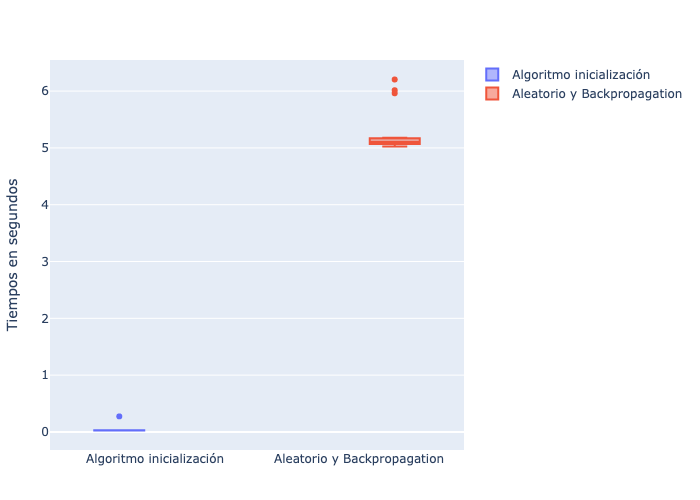
\includegraphics[width=\textwidth]{7-algoritmo-inicializar-pesos/experimento/grafico-bigotes-tiempo.png}
     \caption{Gráfico de caja y bigotes del tiempo requerido por el algoritmo de inicialización de pesos y el de \textit{Backpropagation}.}
\end{figure}
\begin{table}[H]
    \centering
    \resizebox{\textwidth}{!}{
    \begin{tabular}{|l|l|l|l|l|l|l|l|l|l|l|l|l|l|l|l|}
    \hline
        Método & Error  1 & Error  2 & Error  3 & Error  4 & Error  5 & Error  6 & Error  7 & Error  8 & Error  9 & Error  10 & Error  11 & Error  12 & Error  13 & Error  14 & Error  15 \\ \hline
        Algoritmo inicialización & 0,016 & 0,016 & 0,018 & 0,017 & 0,009 & 0,016 & 0,021 & 0,015 & 0,018 & 0,020 & 0,016 & 0,016 & 0,016 & 0,019 & 0,018 \\ \hline
        Aleatorio y Backpropagation & 0,582 & 0,570 & 0,570 & 0,575 & 0,564 & 0,567 & 0,564 & 0,567 & 0,572 & 0,570 & 0,561 & 0,561 & 0,574 & 0,569 & 0,563 \\ \hline
    \end{tabular}
    }
    \caption{Error mínimo cuadrático obtenido en entrenamiento tras acabar la ejecución}
    \label{fig07:error-entrenamiento}
\end{table}

Tal y como se planteó el experimento la parada del algoritmo de \textit{Backpropagation} 
pudo producirse por haber alcanzado un error menor que el la red conseguida con el 
algoritmo de inicialización o porque ha estancado su valor.
Sin embargo, al observarse la distribución de los errores en el 
gráfico \ref{img07:error-entrenamiento} y la tabla \ref{fig07:error-entrenamiento} puede observarse que 
el algoritmo de \textit{Backpropagation} se detuvo al alcanzar un 
mínimo local en todos los casos, ya que todos están por encima del error de nuestro algoritmo de inicialización. 

\begin{figure}[H]
    \centering
     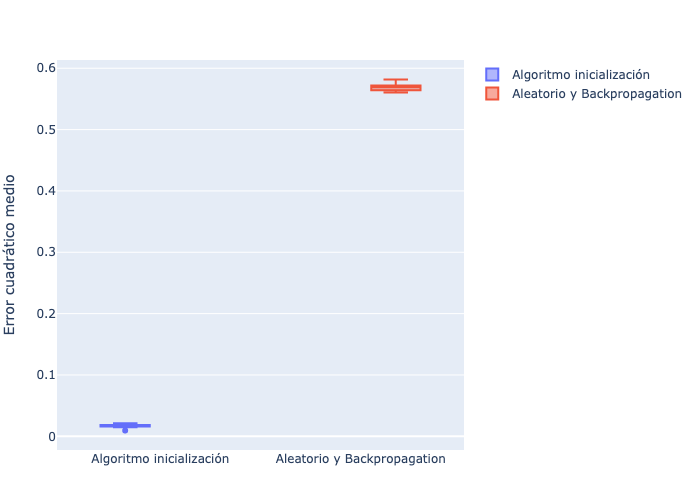
\includegraphics[width=\textwidth]{7-algoritmo-inicializar-pesos/experimento/grafico-bigotes-error_entrenamiento.png}
     \caption{Gráfico de caja y bigotes del \textbf{error en entrenamiento tras finalizar } el algoritmo de inicialización de pesos y el de \textit{Backpropagation}.}
     \label{img07:error-entrenamiento}
\end{figure}

En promedio el error cuadrático medio dentro del entrenamiento conseguido con nuestro algoritmo es 
\begin{equation}
    0,017 \pm 0,003
\end{equation}
mientras que el de inicialización aleatoria y \textit{Backpropagation} es de 
\begin{equation}
    0,569 \pm 0,006. 
\end{equation}

Es interesante entonces comparar el error cuadrático medio obtenido en los datos de test, para ver si efectivamente es tan beneficioso como aparenta el algoritmo creado. 

El resultado en cada ejecución ha sido: 

\begin{table}[H]
    \centering
    \resizebox{\textwidth}{!}{
    \begin{tabular}{|l|l|l|l|l|l|l|l|l|l|l|l|l|l|l|l|}
    \hline
        Método & Error    1 & Error   2 & Error   3 & Error   4 & Error   5 & Error   6 & Error   7 & Error   8 & Error   9 & Error   10 & Error   11 & Error   12 & Error   13 & Error   14 & Error   15 \\ \hline
        Algoritmo inicialización & 0,176 & 0,179 & 0,184 & 0,175 & 0,096 & 0,191 & 0,192 & 0,172 & 0,171 & 0,183 & 0,161 & 0,179 & 0,163 & 0,175 & 0,170 \\ \hline
        Aleatorio y Backpropagation & 0,561 & 0,571 & 0,573 & 0,562 & 0,583 & 0,579 & 0,557 & 0,577 & 0,567 & 0,572 & 0,551 & 0,564 & 0,563 & 0,573 & 0,559 \\ \hline
    \end{tabular}
    }
    \caption{Error mínimo cuadrático \textbf{en test} tras finalizar las sucesivas repeticiones del algoritmo}
\end{table}


\begin{figure}[H]
    \centering
     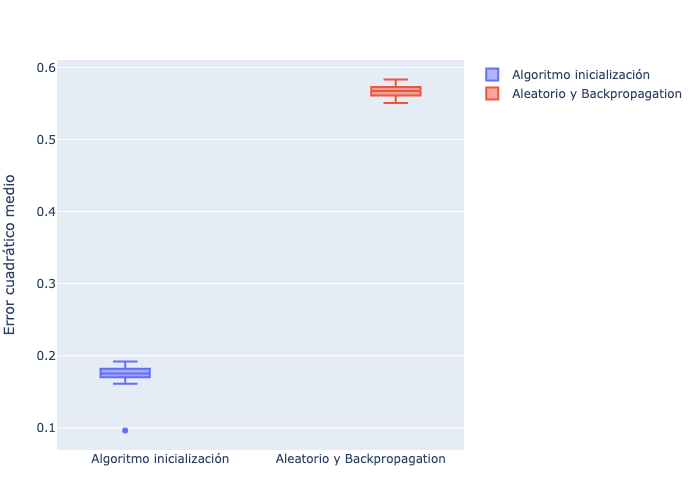
\includegraphics[width=\textwidth]{7-algoritmo-inicializar-pesos/experimento/grafico-bigotes-error_test.png}
     \caption{Gráfico de caja y bigotes del \textbf{error cuadrático medio en test } el algoritmo de inicialización de pesos y el de \textit{Backpropagation}.}
     \label{img07:error-test}
\end{figure}

Donde ahora el promedio para nuestro algoritmo es de un error de
\begin{equation}
    0,171 \pm 0,022
\end{equation}
mientras que el de inicialización aleatoria y \textit{Backpropagation} es de 
\begin{equation}
    0,567 \pm 0,009.
\end{equation}

% Nota sobre sobreajuste 
\marginpar{\maginLetterSize
    \iconoAclaraciones \textcolor{dark_green}{     
        \textbf{
            ¿Qué significa que un modelos está sobreajustado o sobreentrenado?
        }
    }
    En aprendizaje automático un modelo se dice sobreentrenado o sobreajustado 
    cuando ha \textit{aprendido} características 
    propias de los datos de entrenamiento que 
    no son válidas para el problema general. 
    Este efecto produce que se tengan resultados en 
    entrenamiento \textit{mucho} mejores que en test.   
}
Como podemos observar en el caso de nuestro 
algoritmo; a diferencia del error en test obtenido con \textit{Backpropagation}, que el error en test ha superado al de entrenamiento, lo que indica un sobreajuste 
del modelo a los datos de entrenamiento. Esto es totalmente de esperar por 
cómo se construye la inicialización de pesos. Sin embargo, a pesar del sobreajuste, el resultado sigue siendo mejor tanto en precisión como en tiempo que el de aprendizaje usando \textit{Backpropagation}.  



\newpage

